%%%%%%%%%%%%%%%%%%%%%%%%%%%%%%%%%%%%%%%%%%%%%%%%%%%%%%%%%%%%%%%%%%%%%%%%%%%%%%%%%%
\begin{frame}[fragile]\frametitle{}
\begin{center}
{\Large Implementations}
\end{center}
\end{frame}

%%%%%%%%%%%%%%%%%%%%%%%%%%%%%%%%%%%%%%%%%%%%%%%%%%%%%%%%%%%%%%%%%%%%%%%%%%%%%%%%%%
\begin{frame}[fragile]\frametitle{}
\begin{center}
{\Large Agno}
\end{center}
\end{frame}

%%%%%%%%%%%%%%%%%%%%%%%%%%%%%%%%%%%%%%%%%%%%%%%%%%%%%%%%%%%
\begin{frame}[fragile]\frametitle{Introduction to Agno Framework}
      \begin{itemize}
	\item Agno (erstwhile phidata) is a open-source, light-weight framework for building Multi-Agent Systems with memory, knowledge and reasoning
	\item Official documentation available at: \url{https://docs.agno.com/examples/introduction}
	\item Designed for for speed and efficiency and to build production-ready agentic systems with minimal boilerplate
	\item Agno exposes LLMs as a unified API and gives them superpowers like memory, knowledge, tools and reasoning.
	\item Supports 5 progressive levels of agentic system complexity
	\item Framework focuses on performance, reliability, and ease of use
	\item Built for both individual agents and complex multi-agent workflows
	  \end{itemize}
\end{frame}

%%%%%%%%%%%%%%%%%%%%%%%%%%%%%%%%%%%%%%%%%%%%%%%%%%%%%%%%%%%
\begin{frame}[fragile]\frametitle{Key Components}

    \begin{itemize}
	\item Agents: Think in terms of agency and autonomy:
	\item Tools: These are like plugins that give agents extraordinary abilities. 
	\item Memory and Knowledge: Remember past interactions and store relevant information, which allows them to have context and build on previous conversations
Agno also supports connecting to knowledge stores, like Vector databases, to enable retrieval augmented generation (RAG)
	\item Multi-Agent Orchestration: to create teams of agents that can work together
	  \end{itemize}
\end{frame}

%%%%%%%%%%%%%%%%%%%%%%%%%%%%%%%%%%%%%%%%%%%%%%%%%%%%%%%%%%%
\begin{frame}[fragile]\frametitle{The 5 Levels of Agentic Systems}
      \begin{itemize}
	\item \textbf{Level 1:} Agents with tools and instructions - Basic autonomous task execution
	\item \textbf{Level 2:} Agents with knowledge and storage - Persistent data management
	\item \textbf{Level 3:} Agents with memory and reasoning - Context-aware decision making
	\item \textbf{Level 4:} Agent Teams that can reason and collaborate - Multi-agent coordination
	\item \textbf{Level 5:} Agentic Workflows with state and determinism - Complex orchestrated processes
	\item Each level builds upon the previous, enabling progressively sophisticated AI systems
	  \end{itemize}
\end{frame}

%%%%%%%%%%%%%%%%%%%%%%%%%%%%%%%%%%%%%%%%%%%%%%%%%%%%%%%%%%%
\begin{frame}[fragile]\frametitle{Key Features - Model Support \& Performance}
      \begin{itemize}
	\item \textbf{Model Agnostic:} Unified interface to 23+ model providers with no vendor lock-in
	\item \textbf{High Performance:} Agents instantiate in approximately 3 microseconds
	\item \textbf{Memory Efficient:} Uses only 6.5KB memory on average per agent
	\item \textbf{Scalable Architecture:} Designed for production workloads and high throughput
	\item \textbf{Zero Dependencies Overhead:} Minimal resource footprint for deployment
	\item \textbf{Production Ready:} Built-in FastAPI routes for immediate deployment
	  \end{itemize}
\end{frame}

%%%%%%%%%%%%%%%%%%%%%%%%%%%%%%%%%%%%%%%%%%%%%%%%%%%%%%%%%%%
\begin{frame}[fragile]\frametitle{Advanced Capabilities - Reasoning \& Multi-Modal}
      \begin{itemize}
	\item \textbf{Reasoning First-Class:} Three approaches - Reasoning Models, ReasoningTools, custom chain-of-thought
	\item \textbf{Multi-Modal Native:} Accepts text, image, audio, and video inputs
	\item \textbf{Multi-Modal Output:} Generates text, image, audio, and video responses
	\item \textbf{Reliability Focus:} Reasoning improves system reliability for autonomous operations
	\item \textbf{Complex Task Support:} Essential for sophisticated autonomous agent workflows
	\item \textbf{Flexible Implementation:} Choose reasoning approach based on use case requirements
	  \end{itemize}
\end{frame}

%%%%%%%%%%%%%%%%%%%%%%%%%%%%%%%%%%%%%%%%%%%%%%%%%%%%%%%%%%%
\begin{frame}[fragile]\frametitle{Enterprise Features - Search, Memory \& Storage}
      \begin{itemize}
	\item \textbf{Built-in Agentic Search:} Runtime information retrieval using 20+ vector databases
	\item \textbf{State-of-the-art RAG:} Fully asynchronous and highly performant retrieval
	\item \textbf{Long-term Memory:} Built-in Storage \& Memory drivers for persistent context
	\item \textbf{Session Storage:} Maintain conversation state across interactions
	\item \textbf{Structured Outputs:} Fully-typed responses using model structured outputs or JSON mode
	\item \textbf{Real-time Monitoring:} Track agent sessions and performance on agno.com
	  \end{itemize}
\end{frame}

%%%%%%%%%%%%%%%%%%%%%%%%%%%%%%%%%%%%%%%%%%%%%%%%%%%%%%%%%%%
\begin{frame}[fragile]\frametitle{Installation \& Quick Start}
      \begin{itemize}
	\item \textbf{Simple Installation:} Single pip command for complete setup
	\item \textbf{No Complex Dependencies:} Minimal requirements for basic functionality
	\item \textbf{Quick Deployment:} 0 to production in minutes with pre-built routes
	\item \textbf{Extensible Design:} Add tools and capabilities as needed
	\item \textbf{Documentation:} Comprehensive examples and guides available
	  \end{itemize}
      
      \begin{lstlisting}[language=bash]
pip install -U agno
      \end{lstlisting}
\end{frame}

%%%%%%%%%%%%%%%%%%%%%%%%%%%%%%%%%%%%%%%%%%%%%%%%%%%%%%%%%%%
\begin{frame}[fragile]\frametitle{recap: What is an Agent?}

\begin{center}
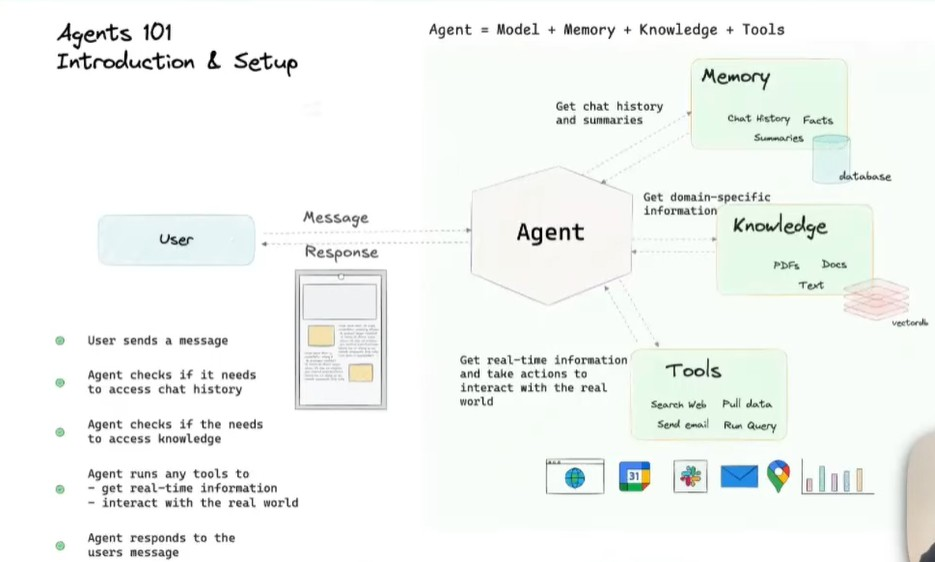
\includegraphics[width=0.8\linewidth,keepaspectratio]{agno1}

{\tiny (Ref: Agents 101 - Agno channel)}
\end{center}	  
\end{frame}

%%%%%%%%%%%%%%%%%%%%%%%%%%%%%%%%%%%%%%%%%%%%%%%%%%%%%%%%%%%
\begin{frame}[fragile]\frametitle{Level 1 Agent Example - Basic Setup}
      \begin{itemize}
	\item Basic reasoning agent with YFinance API integration
	\item Uses Claude Sonnet 4 model for advanced reasoning capabilities
	\item Incorporates ReasoningTools for structured thinking process
	\item YFinanceTools provide stock market data access
	\item Markdown output for formatted responses
	\item Table formatting for clear data presentation
	  \end{itemize}
      
      \begin{lstlisting}[language=python, basicstyle=\tiny]
from agno.agent import Agent
from agno.models.anthropic import Claude
from agno.tools.reasoning import ReasoningTools
from agno.tools.yfinance import YFinanceTools

reasoning_agent = Agent(
    model=Claude(id="claude-sonnet-4-20250514"),
    tools=[
        ReasoningTools(add_instructions=True),
        YFinanceTools(stock_price=True, 
                     analyst_recommendations=True, 
                     company_info=True, company_news=True),
    ],
    instructions="Use tables to display data.",
    markdown=True,
)
      \end{lstlisting}
\end{frame}

%%%%%%%%%%%%%%%%%%%%%%%%%%%%%%%%%%%%%%%%%%%%%%%%%%%%%%%%%%%
\begin{frame}[fragile]\frametitle{Complete Reasoning Agent Implementation}
      \begin{itemize}
	\item Full implementation showing agent creation and execution
	\item Multiple instruction types for behavior control
	\item Stream processing with intermediate step visibility
	\item Full reasoning transparency for debugging and understanding
	\item Real-time output streaming for user engagement
	\item Clean report generation without extraneous text
	  \end{itemize}
      
      \begin{lstlisting}[language=python, basicstyle=\tiny]
from agno.agent import Agent
from agno.models.anthropic import Claude
from agno.tools.reasoning import ReasoningTools
from agno.tools.yfinance import YFinanceTools

agent = Agent(model=Claude(id="claude-sonnet-4-20250514"),
    tools=[ReasoningTools(add_instructions=True),
           YFinanceTools(stock_price=True, analyst_recommendations=True,
                        company_info=True, company_news=True)],
    instructions=["Use tables to display data",
                 "Only output the report, no other text"],
    markdown=True,)

agent.print_response("Write a report on NVDA",
                    stream=True, show_full_reasoning=True,stream_intermediate_steps=True)
      \end{lstlisting}
\end{frame}

%%%%%%%%%%%%%%%%%%%%%%%%%%%%%%%%%%%%%%%%%%%%%%%%%%%%%%%%%%%
\begin{frame}[fragile]\frametitle{Multi-Agent Teams - Architecture Principles}
      \begin{itemize}
	\item \textbf{Atomic Agents:} Individual agents work best with narrow scope and limited tools
	\item \textbf{Specialization:} Each agent focuses on specific domain expertise
	\item \textbf{Load Distribution:} Teams spread cognitive load across multiple agents
	\item \textbf{Scalable Design:} Handle multiple concepts through agent collaboration
	\item \textbf{Tool Management:} Prevent tool overload by distributing capabilities
	\item \textbf{Coordinated Execution:} Team-level orchestration for complex tasks
	  \end{itemize}
\end{frame}

%%%%%%%%%%%%%%%%%%%%%%%%%%%%%%%%%%%%%%%%%%%%%%%%%%%%%%%%%%%
\begin{frame}[fragile]\frametitle{Multi-Agent Team Implementation - Part 1}
      \begin{itemize}
	\item Web Agent specializes in information search and sourcing
	\item Finance Agent focuses on financial data retrieval and analysis
	\item Each agent has dedicated tools for their domain
	\item Domain-specific instructions optimize agent behavior
	  \end{itemize}
      
      \begin{lstlisting}[language=python, basicstyle=\tiny]
from agno.agent import Agent
from agno.models.openai import OpenAIChat
from agno.tools.duckduckgo import DuckDuckGoTools
from agno.tools.yfinance import YFinanceTools

web_agent = Agent(name="Web Agent",
    role="Search the web for information",
    model=OpenAIChat(id="gpt-4o"),
    tools=[DuckDuckGoTools()],
    instructions="Always include sources",
    show_tool_calls=True, markdown=True,)

finance_agent = Agent(name="Finance Agent", role="Get financial data",
    model=OpenAIChat(id="gpt-4o"),
    tools=[YFinanceTools(stock_price=True, 
                        analyst_recommendations=True,
                        company_info=True)],
    instructions="Use tables to display data",
    show_tool_calls=True, markdown=True,)
      \end{lstlisting}
\end{frame}

%%%%%%%%%%%%%%%%%%%%%%%%%%%%%%%%%%%%%%%%%%%%%%%%%%%%%%%%%%%
\begin{frame}[fragile]\frametitle{Multi-Agent Team Implementation - Part 2}
      \begin{itemize}
	\item Team coordination mode enables collaborative agent interaction
	\item Stream processing provides real-time team collaboration visibility
	\item Comprehensive reporting combines multiple agent capabilities
	\item \lstinline|pip install ddgs yfinance|
	  \end{itemize}
      
      \begin{lstlisting}[language=python, basicstyle=\tiny]
from agno.team import Team
	  
agent_team = Team(
    mode="coordinate",
    members=[web_agent, finance_agent],
    model=OpenAIChat(id="gpt-4o"),
    success_criteria="A comprehensive financial news report with clear sections and data-driven insights.",
    instructions=["Always include sources", 
                 "Use tables to display data"],
    show_tool_calls=True,
    markdown=True,)

agent_team.print_response(
    "What's the market outlook and financial performance of AI semiconductor companies?", 
    stream=True)

      \end{lstlisting}
\end{frame}

%%%%%%%%%%%%%%%%%%%%%%%%%%%%%%%%%%%%%%%%%%%%%%%%%%%%%%%%%%%
\begin{frame}[fragile]\frametitle{Performance Philosophy \& Benchmarking}
      \begin{itemize}
	\item \textbf{Performance by Design:} Agents optimized for speed and efficiency from ground up
	\item \textbf{Accuracy Priority:} Reliability and correctness more important than raw speed
	\item \textbf{Fair Benchmarking:} Framework differences make direct comparisons challenging
	\item \textbf{Self-Comparison Focus:} Future benchmarks will compare against previous Agno versions
	\item \textbf{Continuous Optimization:} Performance tuning is ongoing development priority
	\item \textbf{Production Metrics:} Real-world performance measurement over synthetic benchmarks
	  \end{itemize}
\end{frame}

%%%%%%%%%%%%%%%%%%%%%%%%%%%%%%%%%%%%%%%%%%%%%%%%%%%%%%%%%%%
\begin{frame}[fragile]\frametitle{Getting Started - Next Steps}
      \begin{itemize}
	\item \textbf{Start Simple:} Begin with Level 1 agents to understand core concepts
	\item \textbf{Progressive Complexity:} Advance through levels as requirements grow
	\item \textbf{Documentation:} Explore comprehensive examples at docs.agno.com
	\item \textbf{Community Support:} Active community for questions and best practices
	\item \textbf{Production Deployment:} Built-in FastAPI routes for immediate scaling
	\item \textbf{Monitoring Integration:} Use agno.com for real-time system insights
	  \end{itemize}
\end{frame}